As stated in section 4 (Background) of this document, the requirements are to code logic using python on the cloud where the main computation of the algorithm will concur using the neural network libraries currently present in Python, whereas, after the logic has been computed, the end result, which in this case will be verbiage, with correct pronunciation and context, will be then returned to the GUI designed for Android phones which will be present on the local system (users phone).
\begin{figure}[htpb]
    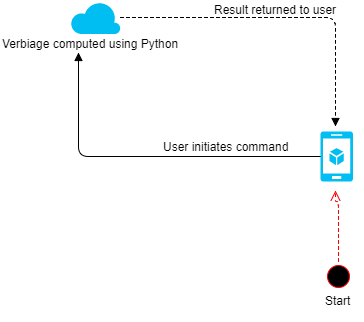
\includegraphics[width=0.8\textwidth]{figures/system-overview}
    \caption{General System Overview}
\end{figure}
The main reason being, one cannot be aware of the computing power of an end users phone, if the computing power is less than what is required by the logic then the application itself will crash. A visual representation is below of the idea behind the system design.
